\chapter{Heuristic Evaluation of Taggle}
\label{chap:heuristiceval}
\ifpdf
    \graphicspath{{Chapters/HeuristicEvaluation/HeuristicEvaluationFigs/PNG/}{Chapters/HeuristicEvaluation/HeuristicEvaluationFigs/PDF/}{Chapters/HeuristicEvaluation/HeuristicEvaluationFigs/}}
\else
    \graphicspath{{Chapters/HeuristicEvaluation/HeuristicEvaluationFigs/EPS/}{Chapters/HeuristicEvaluation/HeuristicEvaluationFigs/}}
\fi  

An inexpensive and popular method for evaluating the usability of an interactive tool is to employ an evaluation using a set of heuristics such as Nielsen's \textit{Ten Usability Heuristics} for user interface design \citep{nielsen92}. In this type of evaluation, a number of experts review a tool and determine how well it follows some predefined guidelines. As part of our overall evaluation strategy, we conducted a heuristic evaluation of interactive tag cloud visualisation tool Taggle using a heuristic set specially designed for information visualisation tools. Subjective user feedback was sought to clarify research questions regarding the comprehensibility of the visualisation technique, as well as assessing the system usability. In \S\ref{sect:heuristics}, we outline the set of heuristics used to evaluate Taggle. The methodology of the evaluation is detailed from \S\ref{sect:heuristicparticipants} through \S\ref{sect:heuristicprocedure}. Results from the heuristics themselves, the guideline checklist and questionnaire are presented in \S\ref{sect:heuristicevalresults}. Finally, subsequent adaptations resulting from the evaluation are presented and summarised in \S\ref{sect:heuristicadaptations} and \S\ref{sect:heuristicconclusion}.

\section{Heuristics}\label{sect:heuristics}

Heuristic evaluation is intended as a ``discount usability engineering'' method as opposed to an expensive user trial, in particular because so few participants are needed. Nielsen's recommendation was to use three to five evaluators since that number is sufficient to identify most of the issues.

Information visualisation tools require a set of heuristics specifically tailored to finding usability issues that focus on the process of data exploration and visualisation techniques. Existing research has identified a number of heuristic sets and guidelines. The well-known `information seeking mantra' by \citet{schneiderman96} guides successful data exploration. \citet{luzzardi04} proposed an extended set of ergonomic criteria for information visualisation techniques which were designed to assess both visualisation and interactivity techniques for hierarchical data representations. \citet{zuk06b} outlined a set of heuristics based on previous theories and principles in perception and cognition by \citet{bertin83}, \citet{tufte90} and \citet{ware04}. Finally, \citet{forsell10} took these and other developed heuristic sets such as \citep{nielsen92} and used empirical methods to synthesize them into a new set of ten heuristics which could provide the widest possible explanatory cover proportionally for all 63 heuristics presented in their study. It is this set of heuristics which was used to evaluate Taggle. Artefacts used in the heuristic evaluation sessions (including a complete description of the heuristics with additional guidelines on how to apply them) are available in Appendix~\ref{app:heartefacts}.

The purpose of the heuristic evaluation was to elicit user feedback which resulted in design refinements, and to check the tool was sufficiently detailed to be used in further trials. Subjective feedback was gained on certain points of interest to help shape tasks for future experiments. In particular, we wished to clarify the following research questions:

\begin{description}
  \item[RQ:]Is the visualisation technique itself instinctively comprehensible? Can the visualisation supply the user with a good overall picture of the data?
  \item[RQ:]Can users infer general information about the data from interacting with the visualisation? What kind of information? 
  \item[RQ:]Is the data mapping process understandable?
  \item[RQ:]Is the supplied system interactivity sufficient for accumulating knowledge about the data? 
\end{description}

By evaluating our software through the use of a heuristic set, we wished to elicit user opinion on the system usability with regards to visual representation, interactivity, flexibility and consistency in design choices.

\section{Participants}\label{sect:heuristicparticipants}
Three evaluators were recruited from Lincoln University and Canterbury University (two female and one male, two academic staff from the Department of Applied Computing and one graduate student from the Department of Computer Science). All evaluators had a solid background in computer science or human computer interaction, and had gained practical and theoretical experience in the field of usability engineering. 

\section{Apparatus}
The evaluations were conducted with the Taggle prototype on a Windows XP PC with 2GB RAM. The 20-inch LCD screen had a resolution of 1680$\times$1050 pixels.

\section{Tag corpora}

Table~\vref{table:datasetheuristiceval} describes the datasets used in the heuristic evaluation. Four datasets were developed, two generic domain datasets and two software engineering. Text fields were sourced from real datasets found online, and in some cases numeric data was artificially generated. 

\begin{table*}
\centering
\caption{\textit{Datasets used in heuristic evaluation}}
\begin{tabular}{|p{2cm}|p{5cm}|p{6cm}|} \hline
\textbf{Data}&\textbf{Columns}&\textbf{Description}\\ \hline
Baby name\par popularity 
& 
Name (text)\par
US popularity (number)\par
NZ popularity (number)\par
&
The popularity rankings are a number between 1\textendash75 representing the popularity ranking of that particular baby name in a given country. For the 75 names represented, the name ranked number 75 is the most popular, and the name ranked number 1 is the least popular. \\ \hline
Software\par metrics
&
Java class name (text)\par
12 software engineering metrics (numeric)\par
&
The software being measured is the open source project jUnit. Twelve metrics have calculated per class, generated by the Sonar software quality platform.\\ \hline
Agile\par development\par stories&
Title (text)\par
Story (text)\par
Actor (text)\par
Estimate in hours (number)\par
&
Describing 35 stories for use in an agile development project for creation of an book store management system. A time figure given in hours has been estimated for the completion of each story.\\ \hline
Cross country challenge
&
Runner ID (number)\par
Surname (text)\par
Club name (text)\par
Score (number)\par
&
The surname and club for 100 runners in a cross country challenge. Each ID pertains to a runner. There are five possible clubs and runners are associated with one club only. The lower score represents a higher placing in the race. \\ \hline
\end{tabular}
\label{table:datasetheuristiceval}
\end{table*}

\section{Procedure}\label{sect:heuristicprocedure}

Each evaluator completed the heuristic evaluation in a separate session which followed the process outlined below:

\begin{enumerate}
	\item Training --- tag clouds and data exploration (5 minutes)
	\item Taggle guided navigation (10 minutes)
	\item Heuristic overview (5 minutes)
	\item Free exploration and issue sheet fill-out (30 minutes) 
	\item Heuristic checklist and questionnaire (10 minutes)
\end{enumerate}

Pre-evaluation, five minutes of training describing tag cloud visualisation using both generic domain and software engineering datasets was given (see Figure~\vref{fig:training} for an example training image used). Evaluators then completed a short tutorial on the Taggle software --- using the same generic dataset, the user was guided through a tour of various interactive features of the software. Participants were given a full and complete description of each heuristic including guidelines on how to apply them (\S\ref{sect:hedescriptions}) and these were then outlined in brief with the opportunity for the evaluator to ask questions.

\begin{figure}[!htb]
	\centering
	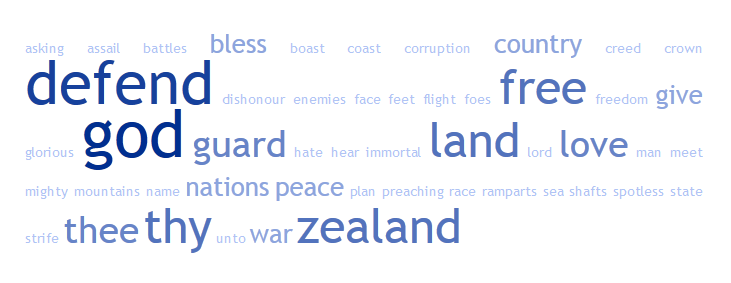
\includegraphics[scale=0.80]{nationalanthem.png}
	\caption{\textit{Training image: tag cloud visualising the New Zealand national anthem. Size and transparency visual properties are used to display word frequency of anthem verses. Stop words such as `is' and `the' have been ignored.}}
	\label{fig:training}
\end{figure}

Following the training sessions, the evaluators were then asked to freely explore Taggle to try to discover information about one or more of the provided datasets. As they explored Taggle, they completed an issue sheet detailing each usability problem found and the severity level. Each evaluator was observed throughout the session and notes taken regarding their comments and suggestions. Evaluators were told to look at any number of the datasets, whichever contained data that was more interesting to them. To take pressure off the analysis, they were also informed that some datasets contained a correlation between data variables, showed an obvious skewed distribution in the data, or contained obvious outliers and that some datasets did not --- there was no `right answer' or any specific data pattern to look for.

Evaluators were also given a sheet of Taggle typical usage patterns (can be found in \S\ref{sect:usagepatterns}) that provided a set of sample tasks for exploration of a dataset. These matched the exact steps taken in the guided navigation tutorial and included steps to set up data mappings, interact with and filter the data, and explore the data to generate hypotheses.

When the evaluator felt that they had learned all they could regarding the chosen dataset or datasets, they then completed a checklist where the evaluator could mark off whether they felt the tool had sufficiently or partially met the recommended guideline for each heuristic. Following this, a questionnaire was completed where evaluators were asked to rate the tool with regards to comprehensibility and knowledge discovery support on a 5-point Likert scale (from 1=``Strongly disagree'' to 5=``Strongly agree'').

\section{Results}\label{sect:heuristicevalresults}

\subsection{Heuristics --- issues, comments and observations}

A complete and full list of usability issues found mapped to the appropriate heuristic with evaluator assigned severity level can be found in \S\ref{sect:heuristicresults}. Figure~\vref{fig:issues} shows the number of issues found per heuristic. This doesn't reflect the total number of issues found, as some issues are related to multiple heuristics.

\begin{figure}[!htb]
	\centering
	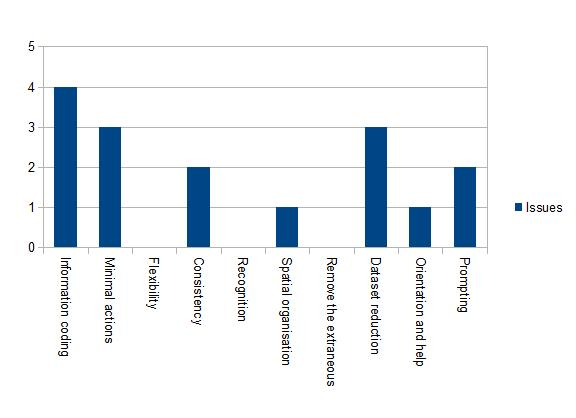
\includegraphics[scale=0.70]{issues.jpg}
	\caption{\textit{Number of issues per heuristic (issues may be related to more than one heuristic)}}
	\label{fig:issues}
\end{figure}

\paragraph{Initial presentation of dataset}
Evaluators thought that the initial starting point when exploring unknown data was confusing. Some users felt that it would be helpful to have the cloud pre-mapped to data fields and a starting cloud displayed on initiation of the software. The default mappings select all options except for transparency. Users felt that starting with just one mapping and adding others as needed was more useful to build knowledge about the dataset.

\paragraph{Selection of data mappings}
The mapping selections were perceived to be the major area which needed improvement. Although not given specific tasks, users quickly ascertained what useful questions might be asked of a dataset (e.g. what club has the best cross country runners?), but had some difficulty selecting mappings that might help them answer these questions. What was useful for decision making in mapping selection was an overview of each variable as a starting point for further investigation (e.g. what is the data range for this variable? Is it text or numerical? Is it categorical?). This information had been provided for them on paper (Table~\vref{table:datasetheuristiceval}), but users commented it would be useful information to integrate into the tool. As a result of initial misunderstandings over data field type, users were sometimes confused by mapping variables to textual data instead of numerical data (this is not useful for mapping to some visual properties such as font size). Conversely, evaluators didn't always map the text label to the tag text but used an numeric ID column. While not as immediately/obviously useful as mapping text, this did have the added advantages of maximising space efficiency in the visualisation, minimising the overemphasising effect of long text and allowing the user to gain an overview of the data in the ID column (ranges for example).

Users didn't use the transparency mapping much at all --- it wasn't perceived to be as useful as font size or colour, and some users were confused by the transparency mapping interface. The drop-down box for layout was confusing as it contained layout options that were for layout research purposes. Evaluators didn't change the default colour set much, although one user commented that black and white were the most helpful colour combinations. A suggestion was made for data to be more complemented by the colour legend. It would be useful for categorical data to be displayed as a colour for every category in a data field.

Another feature requested for mapping selection was the reversal of the mappings properties. This was available for the ordering property but not for size or colour. An evaluator noted that data wasn't always best displayed from smallest to largest numeric value.

\paragraph{Static and dynamic filtering}

Most time was spent by users changing mappings rather than filtering data. One user remarked that this was because of the free exploration nature of the evaluation --- if we had asked more specific questions about the dataset, then more time would have been spent filtering the data to a more appropriate subset according to the question.

The mouse wheel filter was a dynamic filter (appearing on static tab). It was suggested that it would be more useful as a static filter --- useful to discover what settings are most appropriate to display --- and should stay observed after the reset/update button click. This option is not known to the user until they select the filter tab. The dynamic filtering interface was problematic for one user as they didn't realise they could select the knobs on the slider.

\paragraph{Visual encoding}

The visualisation itself didn't pose too many problems for the users. One user wasn't aware of the overview right click pop-up because of an oversight in the training. A complaint about typewriter layout was that it created a disjoint in the flow of the data field mapped to order at the end of each row.

\subsection{Heuristics --- guideline checklist}

The guideline checklist can be found in \S\ref{sect:checklist}. Evaluators were asked to mark each guideline specifying whether they considered each criteria fulfilled, not fulfilled, or partially fulfilled. Each figure visualising results of a heuristic presents marks averaged from  evaluators on a scale between zero and one (where zero means the criteria is not fulfilled, and one means the criteria is fulfilled). This section summarises and discusses guideline checklist results for each heuristic.

\begin{figure}[!htb]
\centering
\begin{subfigure}{.5\textwidth}
	\centering
	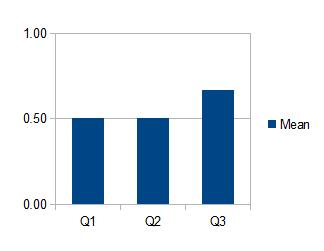
\includegraphics[scale=0.65]{informationcoding.jpg}
\end{subfigure}%
\begin{subfigure}{.5\textwidth}
  \begin{description}
	\item[Q1]Are the data to visual element mappings understandable and effective?
	\item[Q2]Is the use of additional symbols in the representation understandable and effective? 
	\item[Q3]Can you get a general understanding of the underlying data values of an individual item and where the individual data item fits into the overall dataset?
  \end{description}
\end{subfigure}
\caption{\textit{Information coding --- visual representation}}
\label{fig:informationcoding}
\end{figure}

\paragraph{Information coding --- visual representation (Figure~\vref{fig:informationcoding})}

Evaluators felt this criterion was partially fulfilled. One evaluator felt that an overall understanding of the underlying dataset was only possible after a user had some experience or practice with the system. We felt that the responses to this guideline reflected the problems evaluators found with the mapping selection interface. 

\begin{figure}[!htb]
\centering
\begin{subfigure}{.5\textwidth}
	\centering
	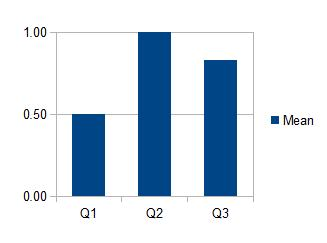
\includegraphics[scale=0.65]{minimalactions.jpg}
\end{subfigure}%
\begin{subfigure}{.5\textwidth}
  \begin{description}
	\item[Q1]Are the number of steps required to perform a task reasonable?
	\item[Q2]For data entry, are currently defined default values displayed in their appropriate data fields?
	\item[Q3]Can the user directly go to a requested view, without having to go through intermediaries?
  \end{description}
\end{subfigure}
\caption{\textit{Minimal actions --- interactivity}}
\label{fig:minactions}
\end{figure}

\paragraph{Minimal actions --- interactivity (Figure~\vref{fig:minactions})}

This criterion was generally satisfied. Issues regarding the number of steps required to perform a task were interpreted as relating to default mapping values and the initial display of the dataset. 

\begin{figure}[!htb]
\centering
\begin{subfigure}{\textwidth}
	\centering
	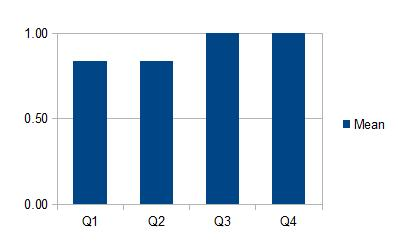
\includegraphics[scale=0.80]{flexibility.jpg}
\end{subfigure}
\begin{subfigure}{\textwidth}
  \begin{description}
	\item[Q1]Are users provided with sufficient means to control visualisation configuration?
	\item[Q2]Are users permitted to define, change or remove default values for settings?
	\item[Q3]When some displays are unnecessary, can users remove or hide them temporarily?
	\item[Q4]Can users change settings in any order?
  \end{description}
\end{subfigure}
\caption{\textit{Flexibility --- interactivity}}
\label{fig:flexibility}
\end{figure}

\paragraph{Flexibility --- interactivity (Figure~\vref{fig:flexibility})}

Evaluators were satisfied that the system provided sufficient flexibility in controlling tag cloud configuration.

\begin{figure}[!htb]
\centering
\begin{subfigure}{\textwidth}
	\centering
	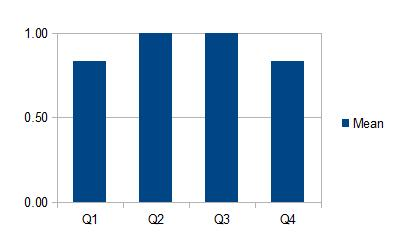
\includegraphics[scale=0.80]{consistency.jpg}
\end{subfigure}
\begin{subfigure}{\textwidth}
  \begin{description}
	\item[Q1]Are window titles always located in the same place?
	\item[Q2]Are the configuration controls consistent?
	\item[Q3]Are similar procedures used to perform tasks?
	\item[Q4]Are labels (phrasing, punctuation, placement) consistent?
  \end{description}
\end{subfigure}
\caption{\textit{Consistency --- interactivity}}
\label{fig:consistency}
\end{figure}

\paragraph{Consistency --- interactivity (Figure~\vref{fig:consistency})}

Criterion was satisfied for consistency in user interface --- configuration controls, window titles, labels and general task procedures. 

\begin{figure}[!htb]
\centering
\begin{subfigure}{.5\textwidth}
	\centering
	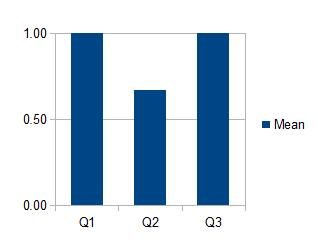
\includegraphics[scale=0.65]{recognition.jpg}
\end{subfigure}%
\begin{subfigure}{.5\textwidth}
  \begin{description}
	\item[Q1]Are the available user actions visible to the user?
	\item[Q2]Can the user perform tasks without having to recall information?
	\item[Q3]Can tasks be performed without referring to external documentation?
  \end{description}
\end{subfigure}
\caption{\textit{Recognition rather than recall --- interactivity}}
\label{fig:recognition}
\end{figure}

\paragraph{Recognition rather than recall --- interactivity (Figure~\vref{fig:recognition})}

This criterion was generally satisfied although evaluators wanted greater access to summary information relating to the dataset.

\begin{figure}[!htb]
\centering
\begin{subfigure}{\textwidth}
	\centering
	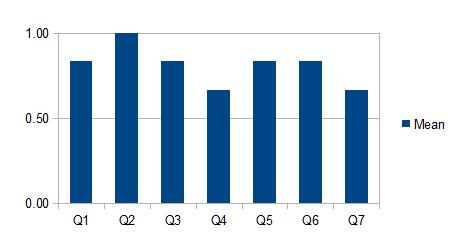
\includegraphics[scale=0.80]{organisation.jpg}
\end{subfigure}
\begin{subfigure}{\textwidth}
  \begin{description}
	\item[Q1]Can I easily locate an information element in the display?
	\item[Q2]Are the individual elements legible?
	\item[Q3]Is space used efficiently in the layout?
	\item[Q4]Am I aware of the overall distribution of information elements in the representation?
	\item[Q5]Are some objects occluded by others?
	\item[Q6]Does the layout follow a logical organisation?
	\item[Q7]Do I understand how tag placement is related to the selected layout and ordering? 
  \end{description}
\end{subfigure}
\caption{\textit{Spatial organisation --- visual representation}}
\label{fig:organisation}
\end{figure}

\paragraph{Spatial organisation --- visual representation (Figure~\vref{fig:organisation})}

Evaluators rated Taggle fairly well for this criteria. One comment regarding the spatial aspect of the visualisation was that the tag cloud could sometimes be very small in the middle of the canvas which wasn't an efficient use of space. This depended on the data mapped though. Another evaluator commented that layout may or may not follow a logical organisation because it depended on their own appropriate mapping selections.

\begin{figure}[!htb]
\centering
\begin{subfigure}{.5\textwidth}
	\centering
	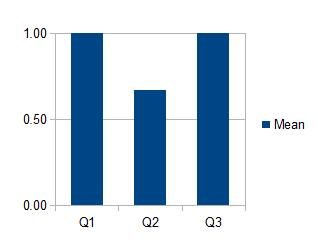
\includegraphics[scale=0.65]{extraneous.jpg}
\end{subfigure}%
\begin{subfigure}{.5\textwidth}
  \begin{description}
	\item[Q1]Are means provided to reduce the distracting effect of extra information when locating information?
	\item[Q2]Are means provided to reduce the distracting effect of extra information when gaining an overview?
	\item[Q3]Are means provided to reduce the distracting effect of extra information when making a comparison?
  \end{description}
\end{subfigure}
\caption{\textit{Remove the extraneous --- interactivity }}
\label{fig:extraneous}
\end{figure}

\paragraph{Remove the extraneous --- interactivity (Figure~\vref{fig:extraneous})}

This criteria was marked as partially met. Evaluators felt that it was important to get a simplified overview of the dataset initially which hadn't been provided for in the interface.

\begin{figure}[!htb]
\centering
\begin{subfigure}{.5\textwidth}
	\centering
	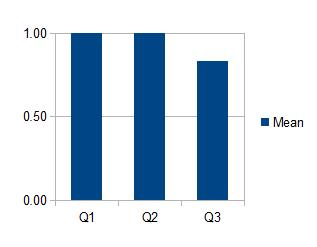
\includegraphics[scale=0.65]{reduction.jpg}
\end{subfigure}%
\begin{subfigure}{.5\textwidth}
  \begin{description}
	\item[Q1]Are means provided to filter/reduce a dataset?
	\item[Q2]Are means provided to ``prune'' or cut off information that may be irrelevant?
	\item[Q3]Are filtering mechanisms efficient and easy to use?
  \end{description}
\end{subfigure}
\caption{\textit{Dataset reduction --- interactivity }}
\label{fig:reduction}
\end{figure}

\paragraph{Dataset reduction --- interactivity (Figure~\vref{fig:reduction})}

Evaluators were satisfied that the system provided sufficient means for filtering and reducing the dataset.

\begin{figure}[!htb]
\centering
\begin{subfigure}{.5\textwidth}
	\centering
	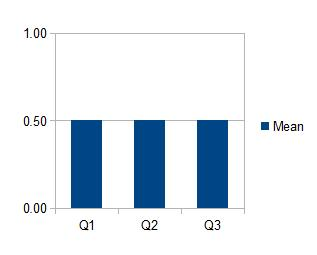
\includegraphics[scale=0.65]{help.jpg}
\end{subfigure}%
\begin{subfigure}{.5\textwidth}
  \begin{description}
	\item[Q1]Are means provided to control levels of detail?
	\item[Q2]Are means provided to redo/undo user actions?
	\item[Q3]Is requested additional information represented, or accessible?
  \end{description}
\end{subfigure}
\caption{\textit{Orientation and help --- interactivity }}
\label{fig:help}
\end{figure}

\paragraph{Orientation and help --- interactivity (Figure~\vref{fig:help})}

Evaluators felt help interactivity was only partially satisfied. More assistance could be provided to orientate the user to the system through means such as redo and undo. 

\begin{figure}[!htb]
\centering
\begin{subfigure}{\textwidth}
	\centering
	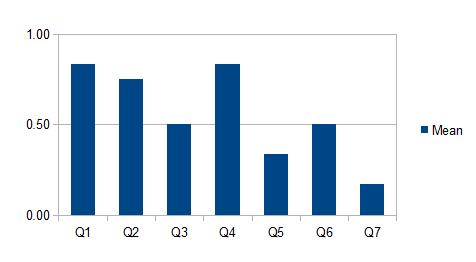
\includegraphics[scale=0.80]{prompting.jpg}
\end{subfigure}
\begin{subfigure}{\textwidth}
  \begin{description}
	\item[Q1]Are users aware of valid values for interface options?
	\item[Q2]Are measurement units displayed for data entry?
	\item[Q3]Is status information displayed?
	\item[Q4]Are labels provided for all fields?
	\item[Q5]Are cues provided on the acceptable length of data entries?
	\item[Q6]Are titles provided for each window?
	\item[Q7]Is online help and guidance provided?
  \end{description}
\end{subfigure}
\caption{\textit{Prompting --- interactivity}}
\label{fig:prompting}
\end{figure}

\paragraph{Prompting --- interactivity (Figure~\vref{fig:prompting})}

As with orientation and help, evaluators felt the prompting status of Taggle could be improved with the addition of things such as online help and more cues on acceptable data entries. We feel manuals and online help guides are more useful and expected for a mature tool rather than a prototype.


\subsection{Questionnaire}

This section presents results for a 5-point Likert scale questionnaire where evaluators were asked to rate the tool with regards to comprehensibility, knowledge discovery support, and other research questions from 1 (``Strongly disagree'') to 5 (``Strongly agree''). Results for each questionnaire section are summarised and discussed.

\begin{figure}[!htb]
\centering
\begin{subfigure}{\textwidth}
	\centering
	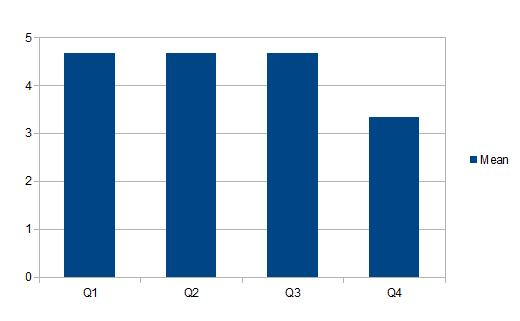
\includegraphics[scale=0.60]{comprehensible.jpg}
\end{subfigure}
\begin{subfigure}{\textwidth}
  \begin{description}
	\item[Q1]I immediately understood that underlying data values between large tags and small tags were different
	\item[Q2]I immediately understood that underlying data values between tags with contrasting colours were different
	\item[Q3]I immediately understood that underlying data values between tags with contrasting transparency levels were different
	\item[Q4]When looking at a visualisation the tag label gave me an immediate visual clue as to the kind of data the tag was representing
  \end{description}
\end{subfigure}
\caption{\textit{Is the visualisation technique instinctively comprehensible?}}
\label{fig:comprehension}
\end{figure}

\paragraph{Is the visualisation technique instinctively comprehensible? (Figure~\vref{fig:comprehension})}

Users agreed or strongly agreed that they could immediately comprehend that tags with contrasting font sizes, colours or transparencies had differing underlying data values. It was observed that evaluators frequently mapped the tag text to numeric fields. This may have contributed to the feeling that the tag label didn't always give an immediate visual clue to the represented data, as this greatly depends on the users choice of mappings.

\begin{figure}[!htb]
\centering
\begin{subfigure}{\textwidth}
	\centering
	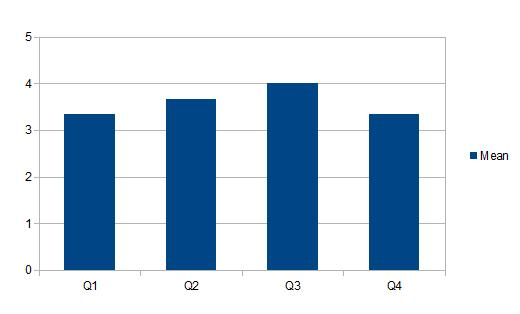
\includegraphics[scale=0.60]{inferinformation.jpg}
\end{subfigure}
\begin{subfigure}{\textwidth}
  \begin{description}
	\item[Q1]I could infer the underlying data distribution of a dataset/datasets 
	\item[Q2]While interacting with the tag cloud, I could identify outliers of a dataset/datasets
	\item[Q3]In a dataset/datasets, I could distinguish which tags had similar (data) characteristics
	\item[Q4]I could distinguish a relationship between one data variable and another data variable
  \end{description}
\end{subfigure}
\caption{\textit{Are users able to infer general information about the data from interacting with the visualisation? What kind of information?}}
\label{fig:inferinformation}
\end{figure}

\paragraph{Are users able to infer general information about the data from interacting with the visualisation? What kind of information? (Figure~\vref{fig:inferinformation})}

All users were able to infer the underlying data distribution (ranging from one dataset to all datasets), although with various levels of difficulty. All users were able to identifier outliers in a dataset and distinguish tags which had similar data characteristics. One evaluator commented they “found it difficult to choose the right mappings ” when trying to distinguish relationships between data variables.

\begin{figure}[!htb]
\centering
\begin{subfigure}{.5\textwidth}
	\centering
	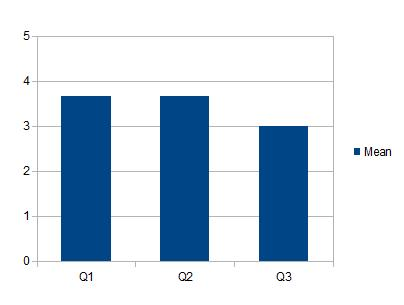
\includegraphics[scale=0.50]{backgroundcolour.jpg}
\end{subfigure}%
\begin{subfigure}{.5\textwidth}
  \begin{description}
	\item[Q1]Tag clouds were easier to read with background colour around the text
	\item[Q2]Background colour around the text enhanced my knowledge of a particular dataset/s
	\item[Q3]I forgot that I could put the colour around the background of the tag 
  \end{description}
\end{subfigure}
\caption{\textit{Does background colour around the text make data easier to understand?}}
\label{fig:backgroundcolour}
\end{figure}

\paragraph{Does background colour around the text make data easier to understand? (Figure~\vref{fig:backgroundcolour})}

Background colour was used minimally and evaluators required prompting about the option of putting background colour around the text. Although once used, most agreed it made the tag cloud easier to read.

\paragraph{Is a spiral or typewriter layout preferred? For what kinds of information?}

Evaluators did not establish a clear preference for spiral or typewriter layout for any particular dataset. The comment was made that ``it really depended on the variables mapped''. One user felt that the spiral layout was useful for finding data with similar characteristics and that the typewriter layout affected user perception unnaturally, with arbitrary points for line breaking creating a disjoint in the data. However typewriter layout was perceived as useful for textual labels that benefited from being displayed in alphabetical order. There was an expectation by one evaluator that data with similar characteristics might cluster together or make exact circles in rows around the centre when using the spiral layout.

\begin{figure}[!htb]
\centering
\begin{subfigure}{.5\textwidth}
	\centering
	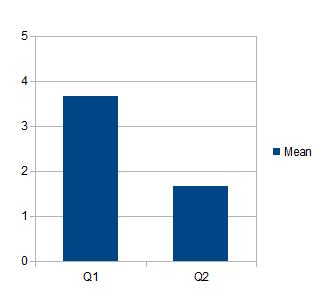
\includegraphics[scale=0.50]{datamapping.jpg}
\end{subfigure}%
\begin{subfigure}{.5\textwidth}
  \begin{description}
	\item[Q1]I found it useful to map a data variable to more than one tag cloud visual feature
	\item[Q2]I didn't try to map a data variable to more than one tag cloud visual feature
  \end{description}
\end{subfigure}
\caption{\textit{Is it useful to map a single data variable to multiple visual features?}}
\label{fig:datamapping}
\end{figure}

\paragraph{Is it useful to map a single data variable to multiple visual features? (Figure~\vref{fig:datamapping})}

All the users tried mapping a single data variable to multiple visual features. Users agreed it was useful to map a single data variable to multiple visual features. When mapping multiple data variables to multiple visual features the comment was made that the tag cloud ``became less useful when mapping more than two data variables''.


% ------------------------------------------------------------------------

%%% Local Variables: 
%%% mode: latex
%%% TeX-master: "../thesis"
%%% End: 


\section{Adaptations resulting from the evaluation}\label{sect:heuristicadaptations}

Having considered the evaluators' responses, we decided to modify Taggle to include some of their more significant suggestions.

\paragraph{Initial presentation of dataset}

Simpler default settings were selected. The background colour option was changed to be the default setting, as users agreed on its usefulness but forgot to use it. Linear mappings were set to be the default. Minimal visual features were mapped on cloud load --- only tag text and order are automatically selected, with font size, colour and transparency mappings deselected. This is so not to overwhelm the user. Taggle was also altered to produce a cloud automatically after dataset selection to provide the user with a useful starting point.

\paragraph{Selection of data mappings}

\begin{figure}[!htb]
\centering
\begin{subfigure}{.5\textwidth}
	\centering
	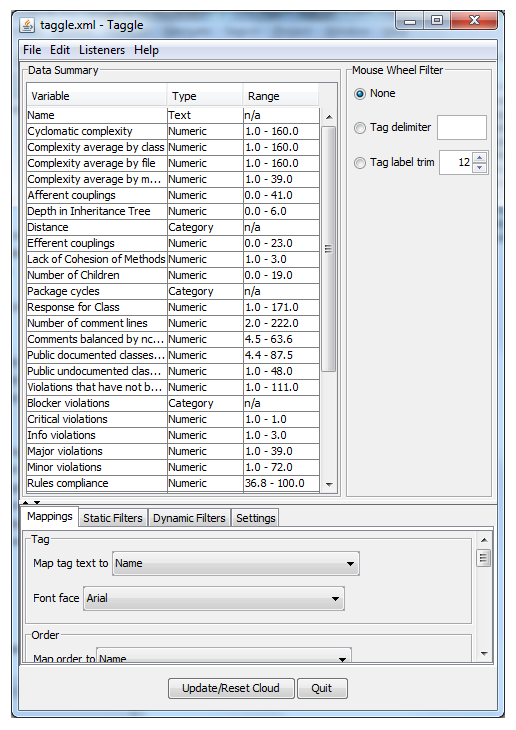
\includegraphics[scale=1.20]{datasummary1.png}
\end{subfigure}%
\begin{subfigure}{.5\textwidth}
	\centering
	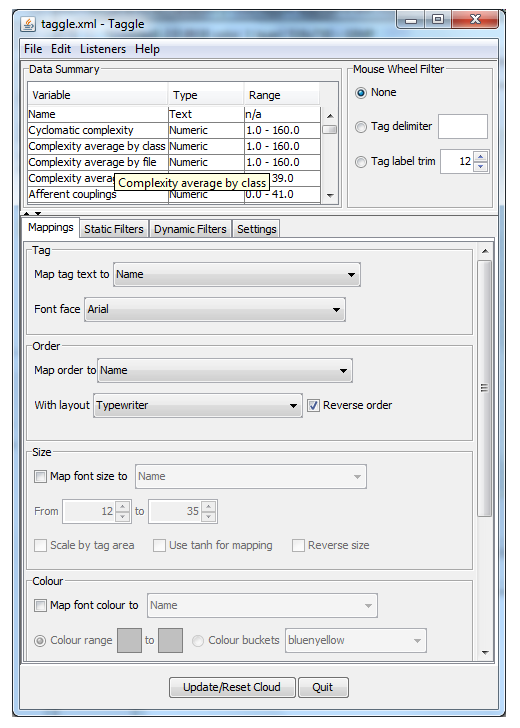
\includegraphics[scale=1.20]{datasummary2.png}
\end{subfigure}
\caption{\textit{Expandable data summary screen}}
\label{fig:datasummaries}
\end{figure}

Evaluators wanted the underlying data field names, ranges and data forms (such as text, number, category) more visible to the user to assist them with mapping selection. Figure~\vref{fig:datasummaries} shows a scrollable, expandable data summary screen which was added above the tabbed panes showing information about each data field. This panel could be visible at all times while selecting mappings or applying filters, but could also be expanded or contracted to match user's preference or knowledge of the dataset.

For mapping selection data entry, editable fields applied rules to help the user make more appropriate choices. For example, the font size maximum spinner buttons were changed to move the minimum font size to always less than the maximum number within the specified absolute minimum/maximum).

Mapping boxes were disabled when dechecked to make it absolutely clear that they were not being applied in the tag cloud. Layout algorithms were better labelled and unused items were disabled to minimise confusion (see Figure~\vref{fig:layout}).

\begin{figure}[!htb]
	\centering
	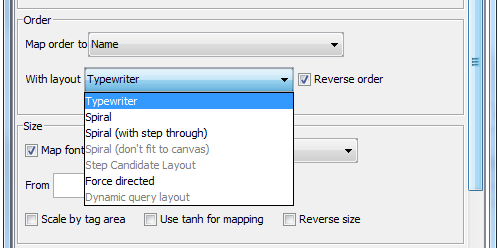
\includegraphics[scale=1.80]{layout.png}
	\caption{\textit{Layout algorithm relabelled}}
	\label{fig:layout}
\end{figure}

Evaluators used colour as a visual mapping property a lot, but were confused about which colour would be appropriate, and tended to use the default settings. It was also noted that the colour mapping was best used for continuous data rather than categorical; colours were presented on a scale with a colour gradient between a minimum and maximum value range. Figure~\ref{fig:colourmapping} shows a change providing an optimal option for categorical data --- colour buckets, where each colour represented a category value. If the mapped data field is categorical then the colour bucket option is automatically selected, otherwise the colour range option is used. For colour buckets, there is a list of colour sets available to use rather than total flexibility in colour choice by user. Colour schemes with appropriate contrast can be entered into an external property file and this will be loaded into the colour bucket drop-down box on Taggle initiation.

\begin{figure}[!htb]
\centering
\begin{subfigure}{\textwidth}
	\centering 
	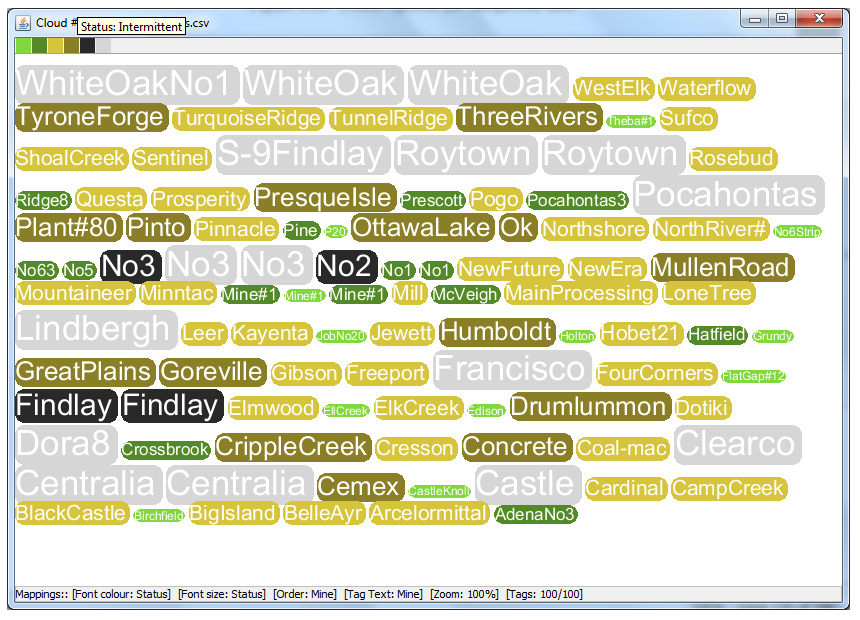
\includegraphics[scale=0.4]{colourmappingcloud.png}
\end{subfigure}
\begin{subfigure}{\textwidth}
	\centering
	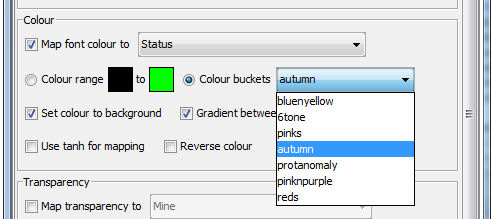
\includegraphics[scale=1.8]{colourmapping.png}
\end{subfigure}
\caption{\textit{Colour options for categorical data --- brown tags are US mines with an operating status of `Intermittent'}}
\label{fig:colourmapping}
\end{figure}

\paragraph{Static and dynamic filtering}

The mouse wheel filtering of the tag text was perceived to the most important filtering option and evaluators requested that the options be more visible to users, especially when performing mapping variable selection. Therefore, these options were moved to the new expandable data summary panel to be viewed at all times (see Figure~\vref{fig:datasummaries}). A third filtering option ``None'' was added, and set to be the default. The maximum label size was renamed a more user-friendly `Tag label trim'. 

\paragraph{Visual encoding}

One aspect of the visual encoding which evaluators wished included was to have categorical data complemented with an associated colour box in the legend. This has been implemented with a fix to the mapping selection colour property (see Figure~\vref{fig:colourmapping}).
 
The overview pop-up in the visual encoding was changed to display on hovering over a tag rather than on right-click, so that it was easier to find.

\section{Summary and discussion}\label{sect:heuristicconclusion}

We felt that through the combination of heuristic issue identification, heuristic guideline checklist, questionnaire and general observation and comment gathering, that we had a reasonable idea of the answers to our initial research questions.

\begin{description}
  \item[RQ:]\textit{Is the visualisation technique itself instinctively comprehensible? Can the visualisation supply the user with a good overall picture of the data?} Users felt they instinctively comprehended that tags with contrasting font sizes, colours or transparencies had differing underlying data values. The tag itself didn't always give an immediate visual clue to represented data as it relied on appropriate user selected mappings.
  \item[RQ:]\textit{Can users infer general information about the data from interacting with the visualisation? What kind of information? } Users were able to infer underlying data distributions, identify outliers and distinguish tags with similar characteristics. This again relied on useful user selected mappings, so difficulty levels varied among evaluators. 
  \item[RQ:]\textit{Is the data mapping process understandable?} Overall, this was the area which evaluators had the most trouble with. Evaluators felt they needed to be supplied with more information about the dataset to support them in choosing appropriate data mappings, since selection of mappings was the most important step in the creation of a cloud which would enable them to refine their knowledge of the underlying data.
  \item[RQ:]\textit{Is the supplied system interactivity sufficient for accumulating knowledge about the data?} There were a number of suggestions made during the heuristic evaluation about how to improve the interactivity of the system. These suggestions were generally around the area of mapping selection. Filtering features were not used extensively in the evaluation --- this could have been improved by providing the evaluators with more specific questions about the given datasets.  
\end{description}

Two of our posed questions in the questionnaire were relating to tag background colour and dual mappings, this served as a initial sanity check for our two planned visual encoding controlled experiments. Tag background colour was agreed to be useful especially when mapping multi-word textual data to the tag label, but as it wasn't set on by default, it wasn't applied until evaluators were reminded that it was an option. Dual mappings for one data field were also perceived as useful when asked. It was commented that multiple mappings for multiple variables became unhelpful when mapping more than two data fields. Based on this primer, we felt confident there were no serious issues in continuing with the planned experiments (presented in Chapters~\ref{chap:exp1}, \ref{chap:exp2}, and \ref{chap:exp3}). As a result of the comments observed and discussed in the heuristic evaluation, a number of adaptations were made to the Taggle prototype in order to improve usability. 


% ------------------------------------------------------------------------


%%% Local Variables: 
%%% mode: latex
%%% TeX-master: "../thesis"
%%% End: 
